\documentclass[tikz,border=10pt]{standalone}
\usepackage{amsmath}
\usetikzlibrary{calc}

\begin{document}

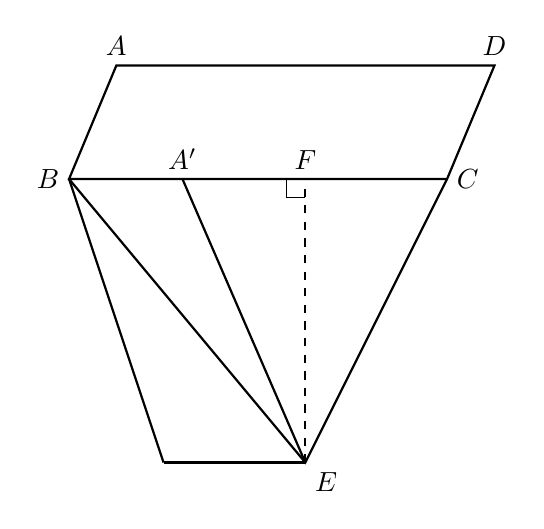
\begin{tikzpicture}[>=stealth, scale=1.2]
    % --- 1. 定义核心顶点坐标 ---
    % 定义平行四边形 ABCD 的顶点
    \coordinate (B) at (0,0);
    \coordinate (C) at (4,0);
    \coordinate (A) at (0.5,1.2);
    \coordinate (D) at ($(A)+(C)-(B)$); % 向量运算保证平行

    % 定义下方延伸点 E (位于 B, C 之外且靠右下方)
    \coordinate (E) at (2.5,-3);

    % 定义 BC 边上的特殊点
    \coordinate (Aprime) at (1.2, 0); % A' 点
    \coordinate (F) at (2.5, 0);      % F 点 (垂足，横坐标同 E)

    % 下方平行的短横线端点
    \coordinate (Eleft) at (1.0,-3);

    % --- 2. 绘制实线路径 ---
    % 绘制上方平行四边形部分区域
    \draw[thick] (A) -- (D) -- (C) -- (B) -- cycle;

    % 绘制下方三角形及连接线
    \draw[thick] (B) -- (E) -- (C);
    \draw[thick] (Aprime) -- (E);
    \draw[thick] (Eleft) -- (E);
    \draw[thick] (B) -- (Eleft); % 连接左侧斜边

    % --- 3. 绘制虚线与辅助要素 ---
    % 绘制垂线 EF
    \draw[dashed, thick] (E) -- (F);

    % 绘制直角符号 (在 F 点)
    \draw (F) ++(0,-0.2) -- ++(-0.2,0) -- ++(0,0.2);

    % --- 4. 标注顶点文字 ---
    \node[above]      at (A) {$A$};
    \node[above]      at (D) {$D$};
    \node[left]       at (B) {$B$};
    \node[right]      at (C) {$C$};
    \node[above]      at (Aprime) {$A'$};
    \node[above]      at (F) {$F$};
    \node[below right] at (E) {$E$};

\end{tikzpicture}

\end{document}